%  use 
%    xdvi -paper usr formulae &
%  and 
%    dvips -t landscape formulae
%  to preview and make PostScript
%,

\documentclass[letterpaper,10pt]{article}

\usepackage{multicol}
\usepackage{calc}
\usepackage{ifthen}
\usepackage{geometry}
\usepackage{amssymb}
\usepackage{amsmath}
\usepackage{graphicx}
\usepackage{titlesec}
\usepackage{color}
\usepackage{listings}
\usepackage{caption}
\usepackage{fancyhdr}
\usepackage{bm}
\usepackage{setspace}
\usepackage{pxfonts}
\usepackage{times}
\usepackage[protrusion=true,expansion=true]{microtype}
\usepackage{hyperref}
\usepackage{lastpage}
\usepackage{mathrsfs}
\usepackage{booktabs}
\usepackage{datetime}
\yyyymmdddate

%\def\thechapter       {\arabic{chapter}}
\def\thesection       {\arabic{section}}
\def\thesubsection    {\alph{subsection}}

\titleformat{\section}
	{\large\bfseries}
	{\thesection.}
	{5pt}
	{}
	{}
	{}

\titleformat{\subsection}
	{\normalsize\bfseries}
	{\hspace{5pt}\thesubsection)}
	{5pt}
	{}
	{}
	{}
	{}

\titleformat{\subsubsection}
	{\small\slshape}
	{\thesubsubsection}
	{1em}
	{}
	{}
	{}

\titlespacing*{\section}      {0pt}{20pt}{0pt}
\titlespacing*{\subsection}   {0pt}{20pt}{10pt}
\titlespacing*{\subsubsection}{0pt}{0pt}{0pt}

\newenvironment{myindentpar}[1]
{\begin{list}{}
	{\setlength{\leftmargin}{#1}}
	\setlength{\parskip}{10pt}
	\item[]
}
{\end{list}}

\renewcommand{\textfraction}{0.05}
\renewcommand{\topfraction}{0.95}
\renewcommand{\bottomfraction}{0.95}
\renewcommand{\floatpagefraction}{0.35}
\setcounter{totalnumber}{5}
\renewcommand{\figurename}{}
\captionsetup{justification=raggedright,
singlelinecheck=false
}

\geometry{top=0.75in,left=0.75in,right=0.75in,bottom=0.75in}
\title{Guidelines for Drawing Ray Diagrams}
%\author{J.L. Lanfranchi, D. Hickstein}
\date{2010.12.16}
\renewcommand{\baselinestretch}{.5}
%\newif\iftechexplorer\techexplorerfalse

%-- Header and footer specification, as per fancyhdr package
\lhead{}
\chead{\fontsize{8}{1}{\hspace{10pt}}\selectfont\scshape Guidelines for Drawing Ray Diagrams{\hfill\vline\hfill}Justin Lanfranchi{\hfill\vline\hfill}2010\,.\,12\,.\,16{\hfill\vline}\hspace{10pt}Page \thepage of \pageref{LastPage}\hspace{10pt}}
\rhead{}
\lfoot{\small\url{http://personal.psu.edu/jll1062/Documents/ray_diagram_howto.pdf}}
\cfoot{}
\rfoot{\small Version 1.1, compiled \today $\,$ \currenttime}
\renewcommand{\headrulewidth}{0.5pt}
\renewcommand{\footrulewidth}{0.5pt}

\newenvironment{mydescription}
{\begin{description}
	\setlength{\itemsep}{0pt}
	\setlength{\parskip}{0pt}
	\setlength{\parsep}{-1pt}}
{\end{description}}
\newenvironment{myitemize}
{\begin{itemize}
	\setlength{\itemsep}{-1pt}
	\setlength{\parskip}{0pt}
	\setlength{\parsep}{0pt}}
{\end{itemize}}

\lstset{
         basicstyle=\footnotesize\ttfamily, % Standardschrift
         numbers=left,               % Ort der Zeilennummern
         numberstyle=\tiny,          % Stil der Zeilennummern
         stepnumber=5,               % Abstand zwischen den Zeilennummern
         numbersep=10pt,              % Abstand der Nummern zum Text
         tabsize=2,                  % Groesse von Tabs
         extendedchars=true,         %
         breaklines=true,            % Zeilen werden Umgebrochen
         keywordstyle=\color{black},
                frame=b,         
         keywordstyle=[1]\textbf,    % Stil der Keywords
         keywordstyle=[2]\textbf,    %
         keywordstyle=[3]\textbf,    %
         keywordstyle=[4]\textbf,    %\sqrt{\sqrt{}} %
         stringstyle=\color{black}\ttfamily, % Farbe der String
         showspaces=false,           % Leerzeichen anzeigen ?
         showtabs=false,             % Tabs anzeigen ?
         xleftmargin=20pt,
         framexleftmargin=10pt,
         framexrightmargin=10pt,
         framexbottommargin=4pt,
         %backgroundcolor=\color{white},
         showstringspaces=false      % Leerzeichen in Strings anzeigen ?        
 }
 \lstloadlanguages{% Check Dokumentation for further languages ...
         %[Visual]Basic
         %Pascal
         %C
         %C++
         %XML
         %HTML
         %Java
		 python
 }
% \DeclareCaptionFont{blue}{\color{blue}} 

% \captionsetup[lstlisting]{singlelinecheck=false, labelfont={blue}, textfont={blue}}
\DeclareCaptionFont{white}{\color{white}}
\DeclareCaptionFormat{listing}{\colorbox[cmyk]{0.43, 0.35, 0.35,0.01}{\parbox{\textwidth}{\hspace{15pt}#1#2#3}}}
\captionsetup[lstlisting]{format=listing,labelfont=white,textfont=white, singlelinecheck=false, margin=0pt, font={bf,footnotesize}}



\pagestyle{fancyplain}

\begin{document}{
%\twocolumn
\fontsize{10pt}{1}\selectfont
%\maketitle
\raggedright
%\singlespacing
%\onehalfspacing

%\section*{Drawing ray diagrams}
%\setlength{\tabcolsep}{12pt}
\section*{Motivation}
\begin{myindentpar}{20pt}
  %Over the course of learning how to draw ray diagrams, we found it challenging
  %to decipher a single set of rules by which all such diagrams might be drawn.
  %The lack of this tool was ultimately an impediment to building a physical
  %intuition for how lenses form images.
   
  In learning about lenses, lens systems, and drawing their associated ray diagrams, we feel that we met with unnecessary difficulty due to a common approach we encountered for teaching ray diagrams: The student is assumed to already have a physical intuition for how lenses work before going through the process. 
 % This was what we found from such as an experienced instructor, textbooks, and various online resources,
  Due largely to this assumption, we found the explanations of ray diagrams to be ambiguous and not generalizable to all situations.
  And starting with a physical intuition and \textit{then} drawing ray diagrams is opposite to how we learned about lenses, where we found ourselves in need of ray diagrams as a reliable tool to \textit{check} our physical intuition for lenses as we built up this intuition.
  
  A good example of a situation that escaped our intuition and the explanations provided is that of virtual objects.
  These can arise when analyzing a system of lenses by taking one at a time.
  If the first lens, adjacent to and preceding (to the left of) a second lens, produces an image on the opposite side (in our case, to the right) of the second lens, this image is considered a \textit{virtual object} for the second lens.
  (If the image were formed on the left side of the second lens, however, it would become a \textit{real object} for the second lens.)
  The first lens is then ignored and the second lens is analyzed for what image it forms of this virtual object.
  The difficulty here is that the general rule that light rays always be drawn from left to right becomes tricky since the object, usually thought of as a source of light rays, is \textit{already on} the right side of the lens.
  Even this situation, however, is simple to work through and consistent with how real objects behave \textit{given the proper guidelines}.

  Therefore, we felt it would be useful to explain ray diagrams as a single, consistently-applicable set of rules by which the inexperienced practitioner might expect to reliably arrive at the behavior of optical devices (inasmuch as the assumptions of geometrical optics allow).
  It is also our goal to inform instructors of the subject of a different perspective of how some students, if similar to us, will most easily learn the topic.
  
  %What follows is the set of rules that we arrived at for .
  %believe would have helped us to not
  %only consistently create correct ray diagrams, but also to 


  %It should be the
  %ultimate goal that a physical intuition informs the ray diagram, rather than
  %the other way around, but until that point comes, we hope that the rules we
  %outline can keep the beginner from coming to erroneous conclusions about the
  %physics due to an erroneously drawn ray diagram.


  
  %Yet we found no resources that laid out a single set of
  %rules by which all such diagrams might be drawn, and so we spent all too many
  %hours feeling around blindly, performing numerical simulations, and finally
  %checking which blind results agreed with the numerical answers. through by
  %trial-and-error results, and 
  % 
  %And the experienced practitioner 


  %instruction for drawing ray
  %diagrams, provided by both our
  %textbook and the experienced practitioner 

  %it seems
  %that most
  
  %since different
  %interpretations led to different results and we found it difficult to
  %check
  
  
  %The textbook used in our optics class presents a couple of
  %examples but these, due to ambiguity in the explanation and due to our
  %uncertainty (at the time) in how the examples generalized to other
  %situations, did not help us work out problems that differed substantially
  %from those examples.
  % 
  %Further, even an experienced practitioner may find it
  %difficult to enumerate all the rules for drawing ray diagrams since intuition
  %for how lenses work, rather than an explicit set of guidelines, may guide him
  %or her through the process. And we believe that the intuition is best built
  %around universally-applicable rules by which the student can check herself
  %Therefore, we felt that it would be helpful both
  %to first-time practitioners and to teachers of the technique to spell out a
  %general set of rules for drawing ray diagrams.

  The circumstances that we seek to address include positive and negative thin lenses with both real and virtual objects.
  A simple extension is then made to a more general class of lens systems (those described entirely by two principal points and two foci, e.g. thick lenses immersed in a single medium).
  Finally, we address drawing ray diagrams for spherical mirrors.
\end{myindentpar}

%\setlength{\tabcolsep}{12pt}
%\section*{Primer}
%\begin{myindentpar}{20pt}
%\end{myindentpar}

%\setlength{\tabcolsep}{12pt}
\section*{Assumptions}
\begin{myindentpar}{20pt}
  We assume that the observer or screen is meant to be on the right side of the lens.
  Therefore a positive thin lens will have its object focus on the left and image focus on the right.
  Negative thin lenses are opposite---the object focus is on the right and the image focus is on the left.
  Note that thin lenses of both types have foci equidistant from the lens.
  Thick lenses and lens systems are not as simple, but we treat this by example later on.
  The condition that the observer be on the right also requires that, regardless of the details of the lens system, the light rays be drawn from left to right in order to locate the resulting image.

  In practice, though, there \textit{are} situations where rays will be necessarily drawn from \textit{right} to \textit{left}.
  This happens, for example, in finding the aperture stop for a lens system with the observer on the right (which is the configuration described above).
  Also, if one were to merely set up an optical system oppositely to that, with the observer or screen on the left of the lens, light rays will have to be drawn from right to left in order to find the image.
  We do not treat the right-to-left case explicitly within the rules below; however, if such a situation arises, all of the \textit{principles} apply equally but rays are to be drawn right to left (if we hadn't already made that clear) and the object and image foci, as described above, switch places.
\end{myindentpar}

%\setlength{\tabcolsep}{12pt}
\section*{Rules for creating thin-lens ray diagrams}
\begin{myindentpar}{20pt}
  \begin{myitemize}
	\item[0.] Getting started
  		\begin{myitemize}
			\item[a)] Start light rays on the far left. Light rays run from left to right, exclusively.
			\item[b)] Draw the optical axis as a horizontal line.
			\item[c)] Draw the lens as a vertical line.
			  A positive lens is indicated by outward-directed arrows on the ends ($\updownarrow$), while a negative lens is indicated by inward-directed arrows.
			\item[d)] Place and label the foci according to the convention laid out above in the \emph{Assumptions} section.
			  Do not skip labelling the foci; the following rules are dependent upon behavior unique to each focus.
			\item[e)] Place the object.
			  Draw a vertical arrow starting from the optical axis and extending some distance up (or down) from the axis.
  		\end{myitemize}
	  \item[1.] Draw \textbf{Ray 1}, or the object/image-focus ray.
  		\begin{myitemize}
			\item[a)] This ray starts from the left running parallel to the optical axis (horizontal in our picture) and has the \textit{intention} of hitting the tip of the object (if no lens were present).
			  In other words, this ray starts at the \textit{height of the object}.
			  This is a crucial point to heed when dealing with virtual objects.
			\item[b)] When this ray finally hits the lens, it either converges to (for a positive lens) or diverges from (for a negative lens) the image focus.
			  Line up a straight edge with both the point at which the ray intersects the lens and the image focus, and draw the ray along this sloped line from the lens rightwards.
  		\end{myitemize}
	  \item[2.] Draw \textbf{Ray 2}, or the object/object-focus ray.
		\begin{myitemize}
			\item[a)] Starting from the left, this ray intends to intersect both the tip of the object and the object focus.
			  Draw Ray 2 as if this were the case, \textit{up until it strikes the lens}.
			\item[b)] Upon striking the lens, Ray 2 bends to be parallel with the optical axis, so draw the ray as a horizontal line from the lens on out to the right.
  		\end{myitemize}
	  \item[3.] Draw \textbf{Ray 3}, or the central ray.
  		\begin{myitemize}
			\item[] Also draw this ray left to right. It passes through both the tip of the object and the center of the lens, and does \textit{not} change direction, even as it strikes the lens.
  		\end{myitemize}
	\item[4.] Locate the image.
  		\begin{myitemize}
		\item[a)] To make it clear what the observer (or screen) on the right of the lens will experience, cover up everything on the left of the lens.
		\item[b)] From what common point does it look like the rays diverge? Or to what point do the rays converge? If the rays on the right side of the lens are diverging, trace them back to their common intersection.
		  If the rays converge on the right side of the lens, the point where they intersect is the tip of the image formed by the system.
		\item[c)] Draw an arrow perpendicular to the optical axis with its tip at the convergence/divergence point just identified.
		  This is the image formed by the lens.
  		\end{myitemize}
  \end{myitemize}
  
  Finally, there are two situations that could cause confusion given these
  rules. First, if the object falls directly on either the object or image
  focus, the ray corresponding with that focus should simply not be drawn. This
  ray would be vertical and, hence, nonsensical. The image can still be found,
  though, with the two remaining rays.
  
  The second situation arises if the object is coincident with the lens. Given
  this, do not draw the central ray (again, a vertical line would result).
  Drawing the other two rays, one will find that the image matches the object,
  regardless of any other details of the setup---neither concavity nor any
  particular focal distance changes this. (Remember, we're dealing with
  \textit{thin} lenses.)
\end{myindentpar}

%\setlength{\tabcolsep}{12pt}
\section*{An example requiring back tracing}
\begin{myindentpar}{20pt}
  Now we present a pictorial example employing the above rules.
 %\begin{figure}[htb]
 %  \caption{Step 1a---draw the optical axis.}
 % 	{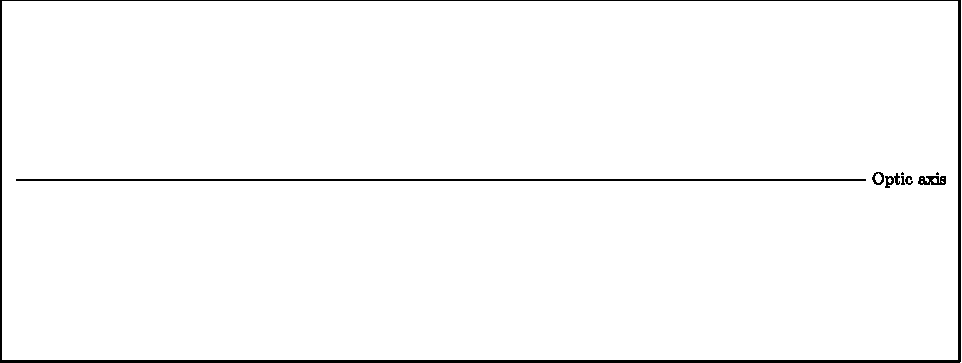
\includegraphics[width=4in,left]{ray_diagram_howto_step01_optic_axis.pdf}}
 %\end{figure}
 %\begin{figure}[htb]
 %   \caption{Step 1b---draw the lens; note that this is a negative lens}
 % 	{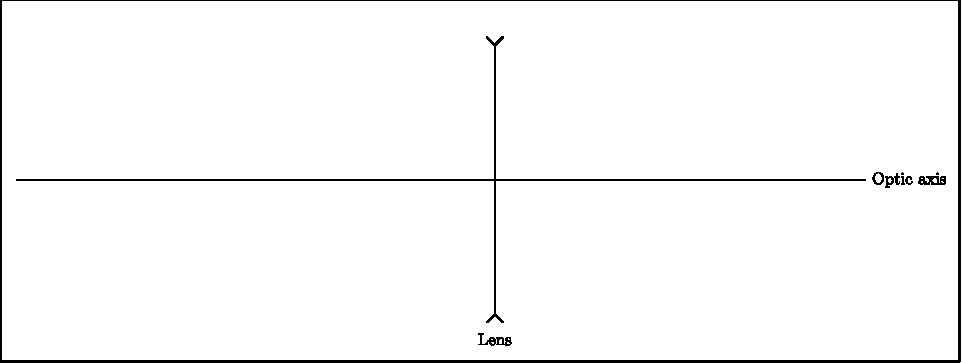
\includegraphics[width=4in,left]{ray_diagram_howto_step02_lens.pdf}}
 %\end{figure}
 \begin{figure}[htb]
	%\caption{Step 1c---label the foci}
   Steps 0a-0d---draw the optical axis, the lens (note this is a negative---aka diverging---lens), and the locations of the foci. \textit{Make sure to label which focus is which!}

  	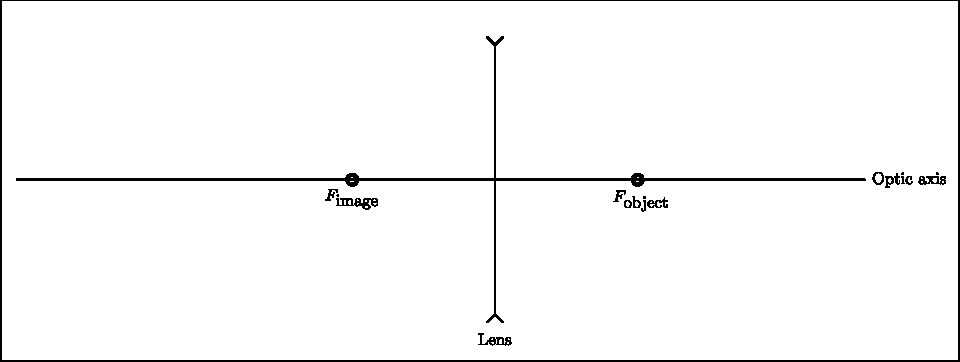
\includegraphics[width=4in,left]{ray_diagram_howto_step03_focii.pdf}
 \end{figure}
 \begin{figure}[htb]
	{Step 0e---draw the object}

  	{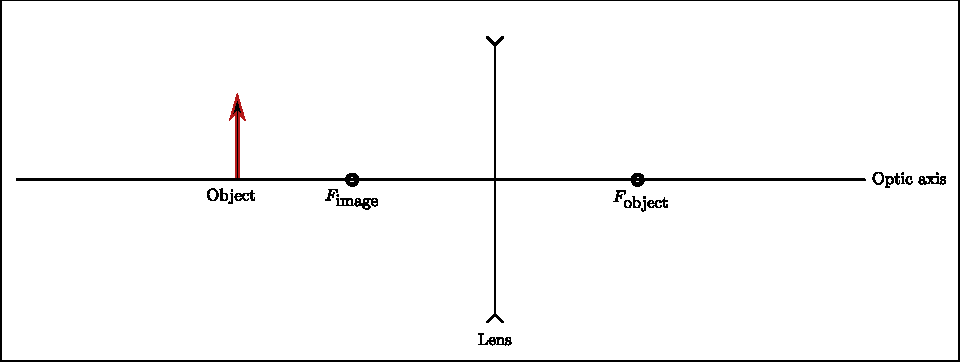
\includegraphics[width=4in,left]{ray_diagram_howto_step04_object.pdf}}
 \end{figure}
 \begin{figure}[htb]
	{Step 1a---Object/image-focus ray (ray 1) starts from left going parallel to OA vertically located so that it (would) hit the object.}

  	{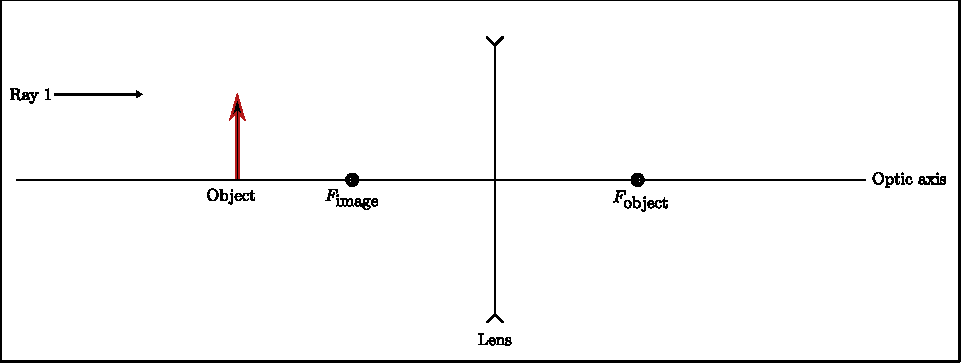
\includegraphics[width=4in,left]{ray_diagram_howto_step05_ray1a.pdf}}
 \end{figure}
 \begin{figure}[htb]
	{Step 1b---Object/image-focus ray (ray 1) continues straight until it hits the lens.}

  	{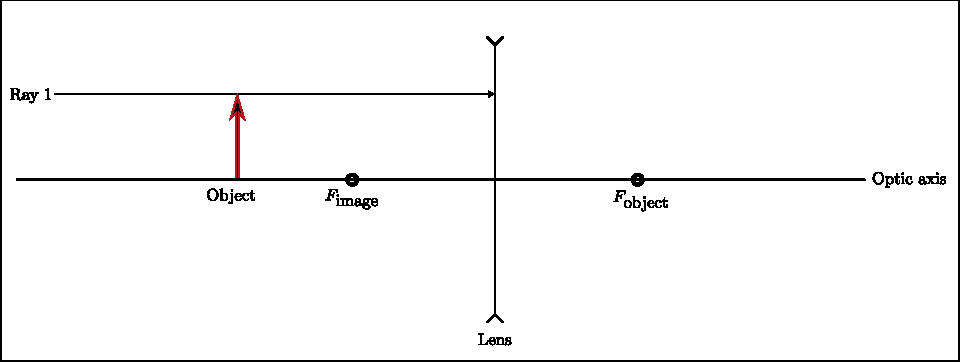
\includegraphics[width=4in,left]{ray_diagram_howto_step06_ray1b.pdf}}
 \end{figure}
 \begin{figure}[htb]
   {Step 1c---Object/image-focus ray (ray 1) bends towards or (as in this case) away from the image focus after hitting the lens. \textit{Note that the dotted line here is just a guide, like where you'd put your ruler and \textbf{not} a traceback!}}

  	{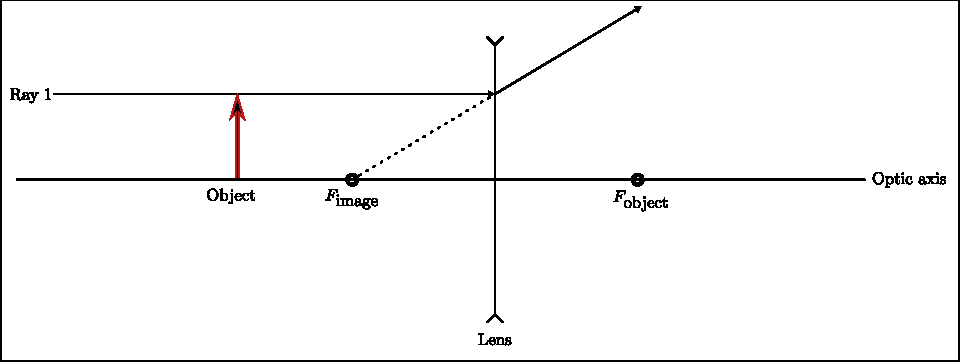
\includegraphics[width=4in,left]{ray_diagram_howto_step07_ray1c.pdf}}
 \end{figure}
 \begin{figure}[htb]
	{Step 2a---Object/object-focus ray (ray 2) starts from the left with ``intention'' to pass through the tip of the object and the object focus. \textit{Note that the dotted line here is just a guide, like where you'd put your ruler and \textbf{not} a traceback!}}

  	{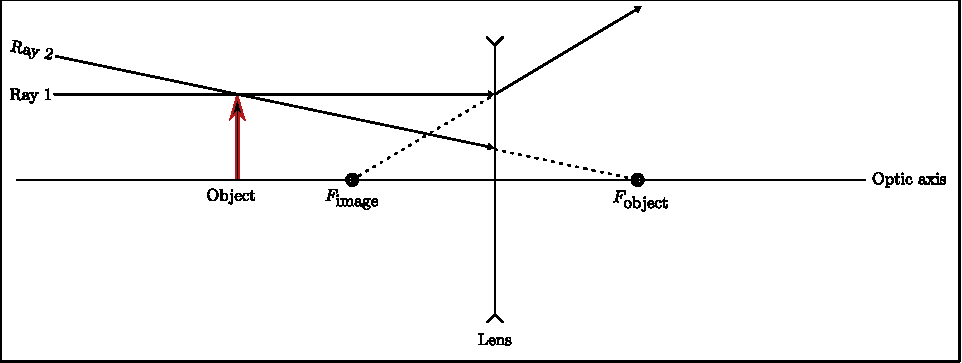
\includegraphics[width=4in,left]{ray_diagram_howto_step08_ray2a.pdf}}
 \end{figure}
 \begin{figure}[htb]
	{Step 2b---Object/object-focus ray (ray 2) bends to parallel upon passing through the lens.}

  	{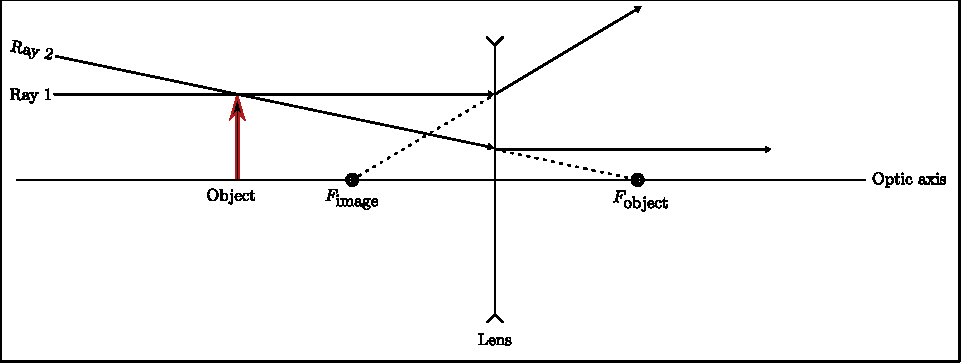
\includegraphics[width=4in,left]{ray_diagram_howto_step09_ray2b.pdf}}
 \end{figure}
 \begin{figure}[htb]
   {Step 3---Central ray (ray 3) passes through the vertex where the lens meets the optical axis, and \textit{does not bend} as it passes through.}

  	{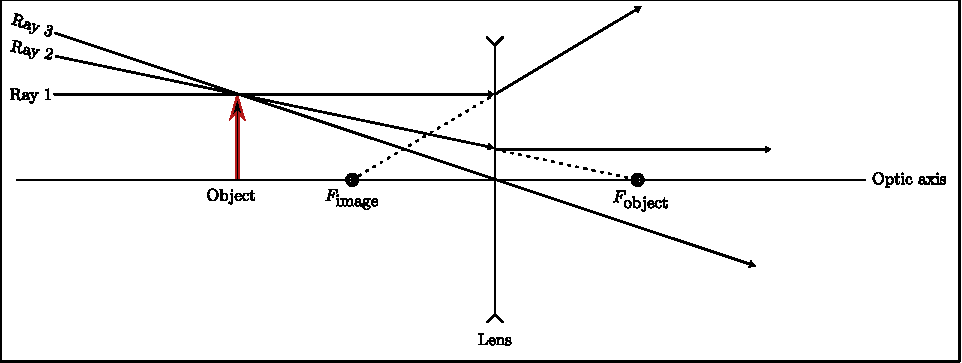
\includegraphics[width=4in,left]{ray_diagram_howto_step10_ray3.pdf}}
 \end{figure}
 \begin{figure}[htb]
   {Step 4a---Cover up the side opposite the observer (the left side in this case); \textit{only pay attention to the rays coming out towards the observer}.}

  	{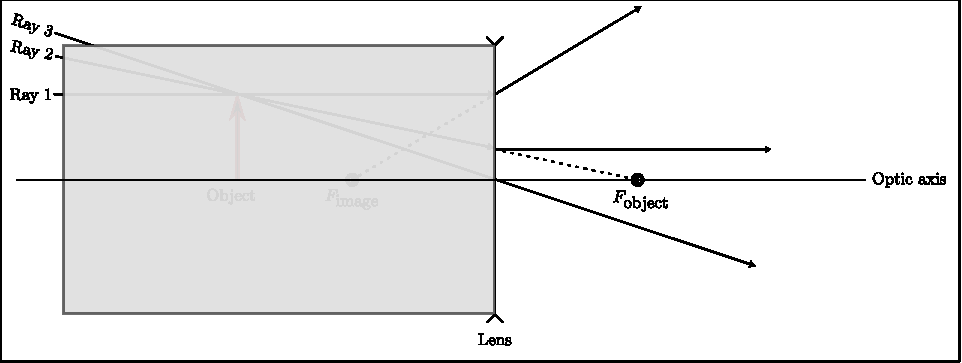
\includegraphics[width=4in,left]{ray_diagram_howto_step11_cover_left.pdf}}
 \end{figure}
 \begin{figure}[htb]
   {Step 4b---Where would an observer perceive the light rays coming from? Identify the rays diverging from a common point on the opposite side of the lens from the observer (as here) or converging to a common point on the same side as the observer.
   The former case, as drawn below, tells you what traceback is necessary (traceback shown as dotted lines).}

  	{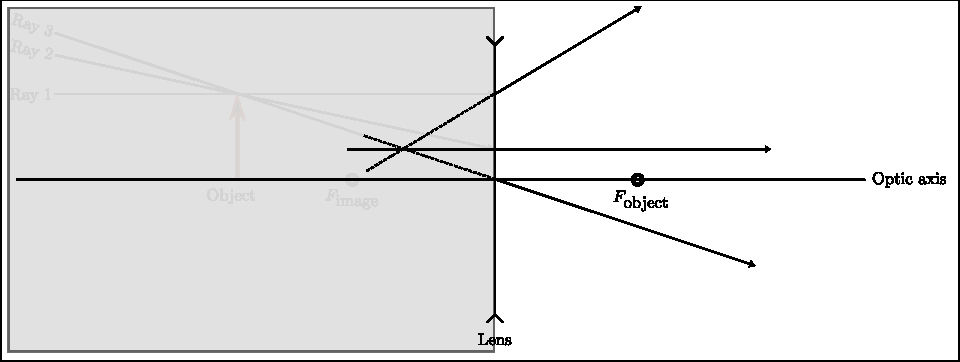
\includegraphics[width=4in,left]{ray_diagram_howto_step12_id_conv_or_div_point.pdf}}
 \end{figure}
 \begin{figure}[htb]
   {Step 4c--Draw an arrow perpendicular to the optical axis with its tip where the lines intersect; this is the image.}

  	{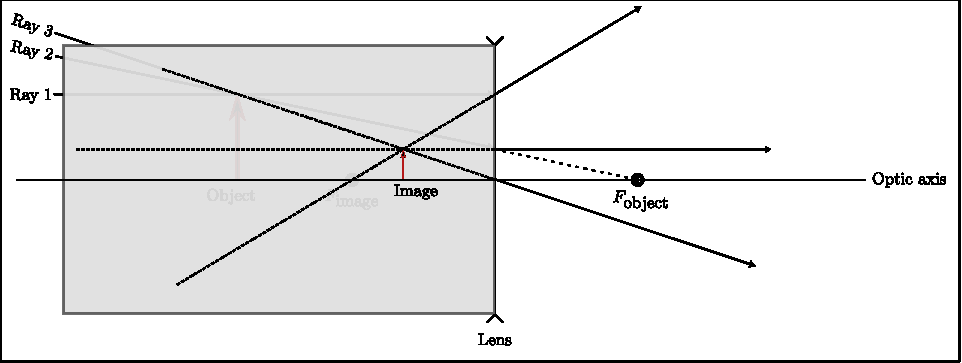
\includegraphics[width=4in,left]{ray_diagram_howto_step13_image.pdf}}
 \end{figure}
 \begin{figure}[htb]
   {Overview of all the lines drawn (as your paper might appear).}

  	{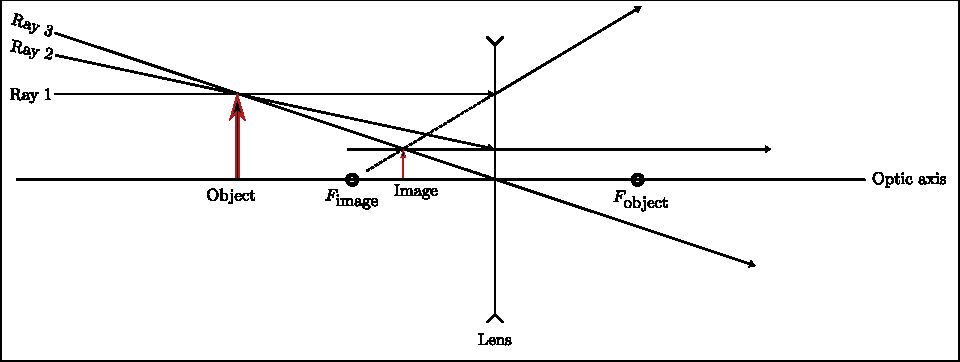
\includegraphics[width=4in,left]{ray_diagram_howto_step14_final.pdf}}
 \end{figure}


\end{myindentpar}



}\end{document}
